\documentclass[border=10pt]{standalone}
\usepackage{tikz}
\usetikzlibrary{positioning, arrows.meta, fit, backgrounds, calc}
\usepackage{xcolor}

% Colors
\definecolor{inputcol}{HTML}{607D8B}
\definecolor{convcol}{HTML}{1976D2}
\definecolor{secol}{HTML}{F57C00}
\definecolor{attncol}{HTML}{388E3C}
\definecolor{fusecol}{HTML}{7B1FA2}
\definecolor{outcol}{HTML}{C62828}
\definecolor{stagebg}{HTML}{F5F5F5}
\definecolor{skipgray}{HTML}{BDBDBD}

\begin{document}
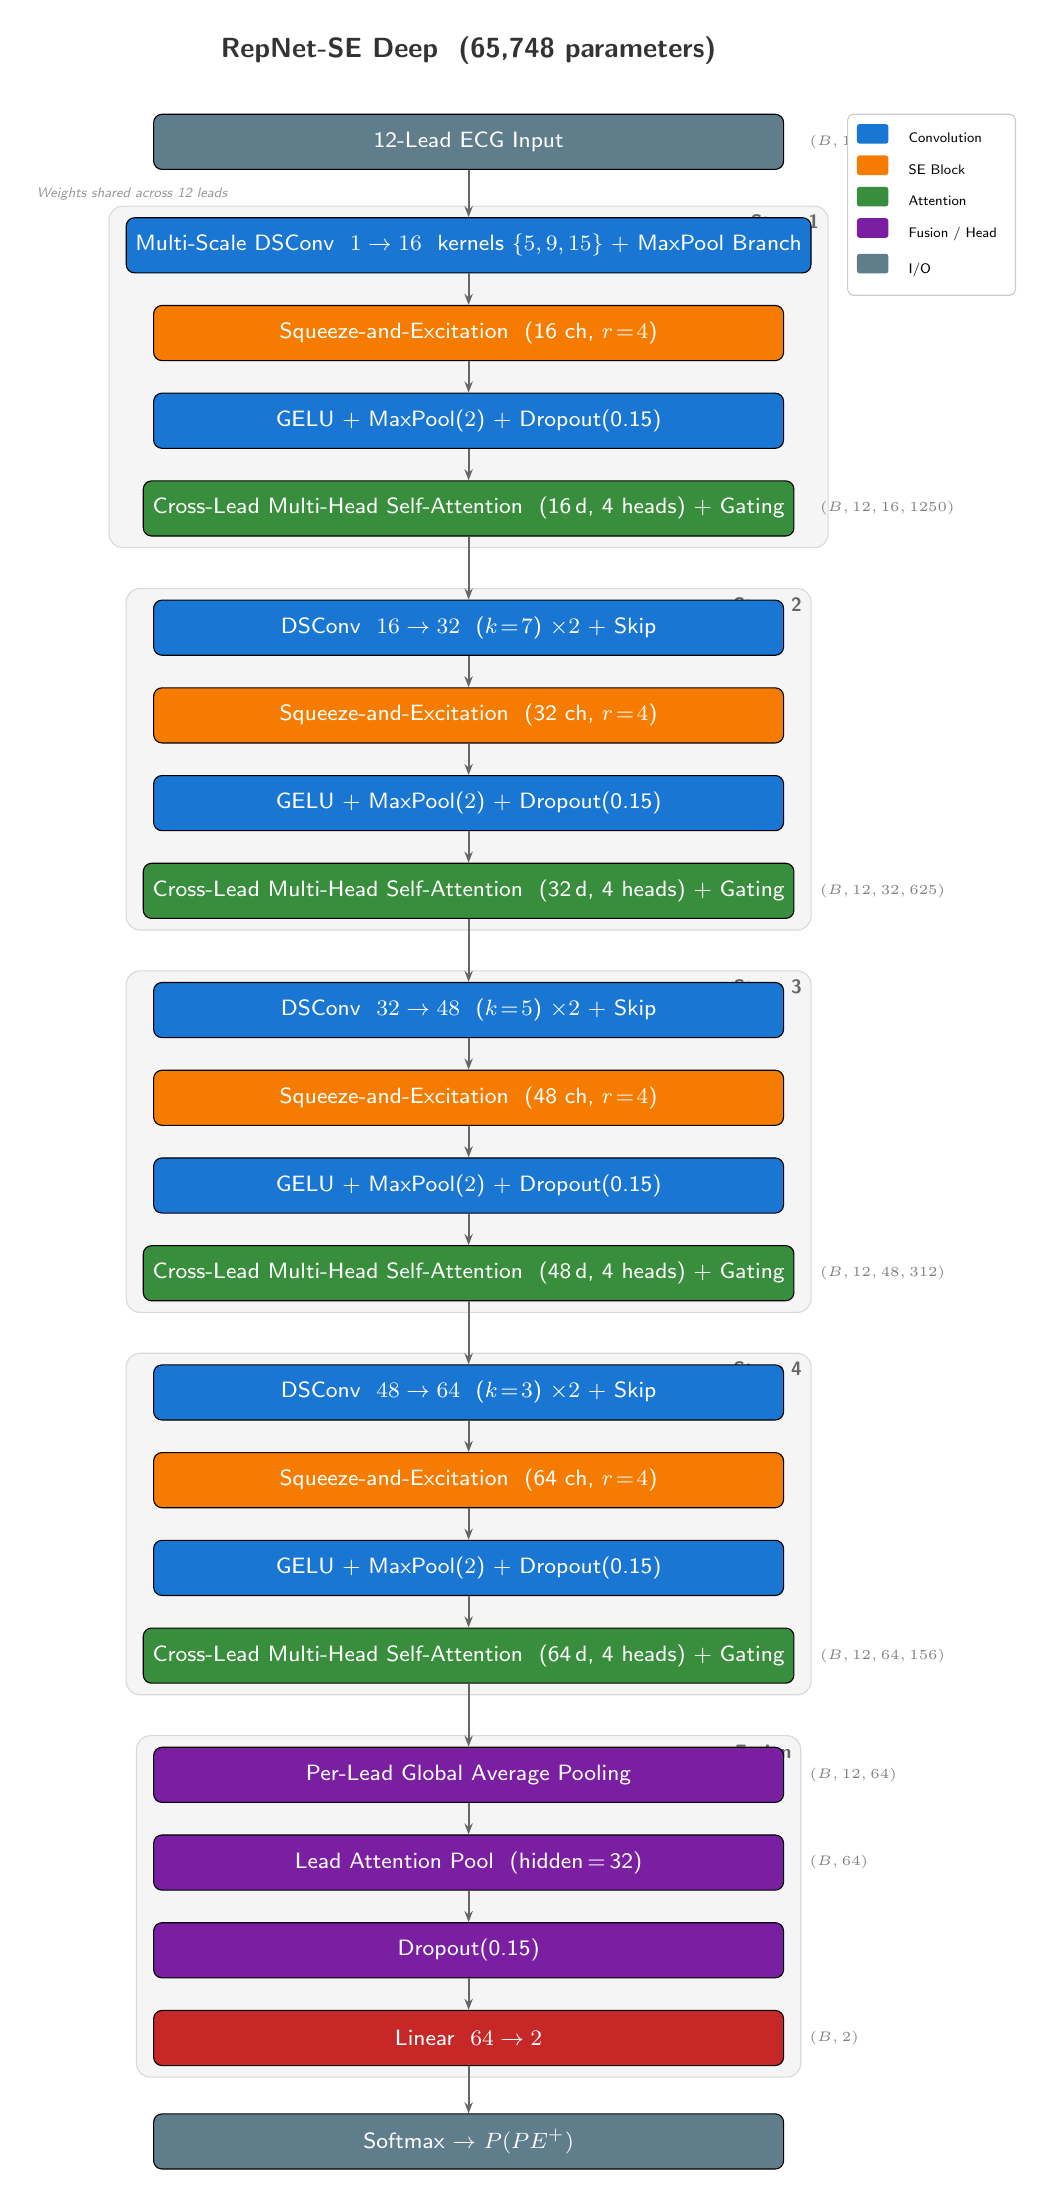
\begin{tikzpicture}[
    node distance=0.4cm and 0cm,
    >={Stealth[length=4pt]},
    block/.style={
        draw, rounded corners=3pt, minimum width=8cm, minimum height=0.7cm,
        font=\footnotesize\sffamily, text=white, align=center,
    },
    convblock/.style={block, fill=convcol},
    seblock/.style={block, fill=secol},
    attnblock/.style={block, fill=attncol},
    fuseblock/.style={block, fill=fusecol},
    ioblock/.style={block, fill=inputcol},
    outblock/.style={block, fill=outcol},
    stagelabel/.style={
        font=\scriptsize\sffamily\bfseries, text=black!60, anchor=north east,
    },
    arrow/.style={->, thick, color=black!60},
    skiparrow/.style={->, thick, color=skipgray, dashed},
    dimtext/.style={font=\tiny\sffamily, text=black!50, anchor=west},
    stagefit/.style={
        draw=black!15, rounded corners=5pt, fill=stagebg,
        inner xsep=6pt, inner ysep=4pt,
    },
]

% ─── Input ───
\node[ioblock] (input) {12-Lead ECG Input};
\node[dimtext, right=0.2cm of input.east] {$(B, 12, 2500)$};

% ─── Stage 1 ───
\node[convblock, below=0.6cm of input] (s1conv)
    {Multi-Scale DSConv~~$1 \to 16$~~kernels $\{5, 9, 15\}$ + MaxPool Branch};
\node[seblock, below=of s1conv] (s1se)
    {Squeeze-and-Excitation~~(16 ch, $r\!=\!4$)};
\node[convblock, below=of s1se] (s1act)
    {GELU + MaxPool($2$) + Dropout(0.15)};
\node[attnblock, below=of s1act] (s1attn)
    {Cross-Lead Multi-Head Self-Attention~~(16\,d, 4 heads) + Gating};
\node[dimtext, right=0.2cm of s1attn.east] {$(B, 12, 16, 1250)$};

% Stage 1 background
\begin{pgfonlayer}{background}
    \node[stagefit, fit=(s1conv)(s1attn), label={[stagelabel]north east:Stage 1}] {};
\end{pgfonlayer}

% ─── Stage 2 ───
\node[convblock, below=0.8cm of s1attn] (s2conv)
    {DSConv~~$16 \to 32$~~($k\!=\!7$) $\times 2$ + Skip};
\node[seblock, below=of s2conv] (s2se)
    {Squeeze-and-Excitation~~(32 ch, $r\!=\!4$)};
\node[convblock, below=of s2se] (s2act)
    {GELU + MaxPool($2$) + Dropout(0.15)};
\node[attnblock, below=of s2act] (s2attn)
    {Cross-Lead Multi-Head Self-Attention~~(32\,d, 4 heads) + Gating};
\node[dimtext, right=0.2cm of s2attn.east] {$(B, 12, 32, 625)$};

\begin{pgfonlayer}{background}
    \node[stagefit, fit=(s2conv)(s2attn), label={[stagelabel]north east:Stage 2}] {};
\end{pgfonlayer}

% ─── Stage 3 ───
\node[convblock, below=0.8cm of s2attn] (s3conv)
    {DSConv~~$32 \to 48$~~($k\!=\!5$) $\times 2$ + Skip};
\node[seblock, below=of s3conv] (s3se)
    {Squeeze-and-Excitation~~(48 ch, $r\!=\!4$)};
\node[convblock, below=of s3se] (s3act)
    {GELU + MaxPool($2$) + Dropout(0.15)};
\node[attnblock, below=of s3act] (s3attn)
    {Cross-Lead Multi-Head Self-Attention~~(48\,d, 4 heads) + Gating};
\node[dimtext, right=0.2cm of s3attn.east] {$(B, 12, 48, 312)$};

\begin{pgfonlayer}{background}
    \node[stagefit, fit=(s3conv)(s3attn), label={[stagelabel]north east:Stage 3}] {};
\end{pgfonlayer}

% ─── Stage 4 ───
\node[convblock, below=0.8cm of s3attn] (s4conv)
    {DSConv~~$48 \to 64$~~($k\!=\!3$) $\times 2$ + Skip};
\node[seblock, below=of s4conv] (s4se)
    {Squeeze-and-Excitation~~(64 ch, $r\!=\!4$)};
\node[convblock, below=of s4se] (s4act)
    {GELU + MaxPool($2$) + Dropout(0.15)};
\node[attnblock, below=of s4act] (s4attn)
    {Cross-Lead Multi-Head Self-Attention~~(64\,d, 4 heads) + Gating};
\node[dimtext, right=0.2cm of s4attn.east] {$(B, 12, 64, 156)$};

\begin{pgfonlayer}{background}
    \node[stagefit, fit=(s4conv)(s4attn), label={[stagelabel]north east:Stage 4}] {};
\end{pgfonlayer}

% ─── Fusion ───
\node[fuseblock, below=0.8cm of s4attn] (gap)
    {Per-Lead Global Average Pooling};
\node[dimtext, right=0.2cm of gap.east] {$(B, 12, 64)$};

\node[fuseblock, below=of gap] (leadpool)
    {Lead Attention Pool~~(hidden\,=\,32)};
\node[dimtext, right=0.2cm of leadpool.east] {$(B, 64)$};

\node[fuseblock, below=of leadpool] (drop)
    {Dropout(0.15)};

\node[outblock, below=of drop] (fc)
    {Linear~~$64 \to 2$};
\node[dimtext, right=0.2cm of fc.east] {$(B, 2)$};

\begin{pgfonlayer}{background}
    \node[stagefit, fit=(gap)(fc), label={[stagelabel]north east:Fusion}] {};
\end{pgfonlayer}

% ─── Output ───
\node[ioblock, below=0.6cm of fc] (output) {Softmax $\to$ $P(\text{PE}^+)$};

% ─── Arrows ───
\foreach \a/\b in {
    input/s1conv, s1conv/s1se, s1se/s1act, s1act/s1attn,
    s1attn/s2conv, s2conv/s2se, s2se/s2act, s2act/s2attn,
    s2attn/s3conv, s3conv/s3se, s3se/s3act, s3act/s3attn,
    s3attn/s4conv, s4conv/s4se, s4se/s4act, s4act/s4attn,
    s4attn/gap, gap/leadpool, leadpool/drop, drop/fc, fc/output%
} {
    \draw[arrow] (\a) -- (\b);
}

% ─── Annotations: shared weights ───
\node[font=\tiny\sffamily\itshape, text=black!40, anchor=west]
    at ($(input.south west) + (-1.6, -0.3)$)
    {Weights shared across 12 leads};

% ─── Legend ───
\matrix[
    draw=black!20, rounded corners=2pt, fill=white,
    column sep=4pt, row sep=1pt,
    anchor=north west,
    font=\tiny\sffamily,
] at ($(input.north east) + (0.8, 0)$) {
    \node[fill=convcol, minimum width=0.4cm, minimum height=0.25cm, rounded corners=1pt] {};
      & \node{Convolution}; \\
    \node[fill=secol, minimum width=0.4cm, minimum height=0.25cm, rounded corners=1pt] {};
      & \node{SE Block}; \\
    \node[fill=attncol, minimum width=0.4cm, minimum height=0.25cm, rounded corners=1pt] {};
      & \node{Attention}; \\
    \node[fill=fusecol, minimum width=0.4cm, minimum height=0.25cm, rounded corners=1pt] {};
      & \node{Fusion / Head}; \\
    \node[fill=inputcol, minimum width=0.4cm, minimum height=0.25cm, rounded corners=1pt] {};
      & \node{I/O}; \\
};

% ─── Title ───
\node[font=\normalsize\sffamily\bfseries, anchor=south, text=black!80]
    at ($(input.north) + (0, 0.5)$)
    {RepNet-SE Deep~~(65,748 parameters)};

\end{tikzpicture}
\end{document}
